\section{Background}\label{sec:background}

\subsection{Soluzioni classiche}
Le tecniche classiche per la rilevazione dei contorni prevedono l'utilizzo di 
kernel specifici, che permettono di calcolare nuovi valori di intensità per i pixel 
dell'immagine. Tra i metodi più famosi vi è sicuramente l'operatore di Sobel, 
che si può descrivere tramite l'applicazione di 2 kernel all'immagine originale:
\[
\mathbf{G_x} =
\begin{bmatrix}
+1 & 0 & -1 \\
+2 & 0 & -2 \\
+1 & 0 & -1
\end{bmatrix}
, \, 
\mathbf{G_y} =
\begin{bmatrix}
+1 & +2 & +1 \\
0 & 0 & 0 \\
-1 & -2 & -1
\end{bmatrix}
\]

Un'altra opzione, forse tra le più utilizzate al giorno d'oggi, è l'operatore di Canny.
Questo metodo ha un funzionamento del tutto analogo al precedente, ma aggiunge 
meccanismi per la riduzione del rumore nell'immagine \cite{digital_image_processing}.
La complessità di queste tecniche è lineare rispetto al numero di pixel totali 
dell'immagine, dato che è necessaria una visita completa. 

Per un'immagine $M \times L = N$, si utilizzano $n$ bit per enumerare i pixel dell'immagine
in formato binario, dove $N = 2^n$, ottenendo una complessità rispetto ai bit esponenziale $\bigo{2^n}$.
In questo progetto verrà mostrato come, dopo una prima fase di preparazione, è possibile risolvere
il problema in tempo costante $\bigo{1}$.

\subsection{Sistemi quantistici}

Analogamente a quanto accade nei computer classici, i computer quantistici utilizzano i \textbf{quantum bit}, chiamati \emph{qubit}. I qubit rappresentano la più piccola unità di informazione e sono implementati attraverso sistemi quantistici bidimensionali. Le quantità fisiche comunemente usate per questo scopo includono lo spin di una particella o gli stati eccitati degli atomi.

Assemblando più qubit, è possibile costruire sistemi quantistici la cui dinamica è descritta da spazi vettoriali complessi. Un sistema composto da un singolo qubit è completamente descritto da
\begin{equation}
	\ket{\psi} = \begin{bmatrix}
		\alpha\\ \beta
	\end{bmatrix} = \alpha \ket{0} + \beta \ket{1},\quad \alpha,\beta \in
	\mathbb{C}
	\label{eq:1-qubit-state}
\end{equation}

Mentre un bit classico può assumere soltanto uno tra due possibili valori
(generalmente 0 e 1), un bit quantistico è denotato da una combinazione lineare
dei suoi stati base, pesata dai coefficienti complessi $\alpha$ e $\beta$. Tali
coefficienti sono detti \emph{ampiezze di probabilità} e rispettano la seguente:
\begin{equation}
	|\alpha|^2 + |\beta|^2 = 1
	\label{eq:qubit-prob}
\end{equation}

Per descrivere lo stato di un sistema quantistico composto da più qubit, è
necessario effettuare un'operazione chiamata \emph{prodotto tensoriale} tra i
singoli stati coinvolti. Ad esempio, considerati i vettori di stati
\[
\ket{\psi_1} = \begin{bmatrix} a_1 \\ a_2 \end{bmatrix}, \quad \ket{\psi_2} = \begin{bmatrix} b_1 \\ b_2 \end{bmatrix},
\]
il loro prodotto tensore è definito come:
\begin{equation}
\ket{\psi_1} \otimes \ket{\psi_2}
= \begin{bmatrix}
a_1 \begin{bmatrix} b_1 \\ b_2 \end{bmatrix} \\
a_2 \begin{bmatrix} b_1 \\ b_2 \end{bmatrix}
\end{bmatrix} =
\begin{bmatrix}
a_1 b_1 \\ a_1 b_2 \\ a_2 b_1 \\ a_2 b_2
\end{bmatrix}.
\label{eq:tensor-prod}
\end{equation}
Equivalentemente, può essere scritto come $\ket{\psi_1}\ket{\psi_2} \text{ o } \ket{\psi_1
\psi_2}$.

\todo{Se serve, parlare dell'entanglement}

\subsection{Circuiti quantistici}

Analogamente a quanto accade nei circuiti digitali classici, i circuiti
quantistici eseguono calcoli manipolando le informazioni immagazzinate nei
qubit. Questo viene realizzato attraverso dispositivi chiamati \textbf{quantum
gate} (\emph{porte quantistiche}), che sono l'equivalente quantistico delle porte logiche classiche
ma operano secondo i principi della meccanica quantistica. L'applicazione di una
matrice \emph{complessa unitaria} ad uno stato quantistico modella matematicamente l'azione di un
gate su di esso. Formalmente, data $U \in \mathcal{M}_{n \times n}(\mathbb{C})$
l'unitaria associata ad una porta logica e dato lo stato $\ket{\psi} \in
\mathbb{C}^n$, lo stato risultante dall'applicazione è definito come:
\begin{equation}
	\ket{\psi'} = U\ket{\psi}
	\label{eq:gate-res-state}
\end{equation}

\subsubsection*{Gate rilevanti}

Di seguito sono descritti alcuni gate quantistici di rilevante importanza. Tra
questi, figurano i \emph{gate di Pauli}.
\begin{itemize}
	\item \textbf{X} (NOT quantistico): trasforma lo stato $\ket{0}$ in $\ket{1}$
	e viceversa;
	\[
		X =\begin{bmatrix}
			0 & 1\\
			1 & 0
		\end{bmatrix}
	\]
	\item \textbf{Y}: combina una rotazione coniugata complessa con un'inversione, utile per applicazioni che coinvolgono trasformazioni nel piano complesso;
	\[
		Y =\begin{bmatrix}
			0 & -i\\
			i & 0
		\end{bmatrix}
	\]
	\item \textbf{Z}: applica una fase negativa allo stato $\ket{1}$ senza influenzare $\ket{0}$.
	\[
		Z =\begin{bmatrix}
			1 & 0\\
			0 & -1
		\end{bmatrix}
	\]
\end{itemize}

Altro gate fondamentale è quello di \emph{Hadamard}\label{txt:hadamard}, essenziale per creare stati
di sovrapposizione. L'unitaria che lo rappresenta è:
\[
	H = \frac{1}{\sqrt 2}\begin{bmatrix}
			1 & 1\\
			1 & -1
		\end{bmatrix}
\]
In particolare, si noti che:
\begin{align}
	H\ket{0} &= \frac{\ket{0} + \ket{1}}{\sqrt 2} =: \ket{+} \\
	H\ket{1} &= \frac{\ket{0} - \ket{1}}{\sqrt 2} =: \ket{-}
\end{align}

Il \emph{Controlled-NOT} (CNOT) è un'operazione che coinvolge due qubit, dove
uno funge da controllo sull'altro. Il gate inverte lo stato del qubit target se il qubit di controllo è $\ket{1}$. La sua matrice è:
\[
	\text{CNOT} = \begin{bmatrix}
		1 & 0 & 0 & 0\\
		0 & 1 & 0 & 0\\
		0 & 0 & 0 & 1\\
		0 & 0 & 1 & 0
	\end{bmatrix}
\]
\subsection{Quantum Image Processing}

La \textbf{Quantum Image Processing} (\emph{processamento quantistico
dell'immagine}) si concentra sullo sviluppo di algoritmi in grado di codificare immagini all’interno di circuiti quantistici e di processarle utilizzando operazioni quantistiche. 

\subsubsection*{Rappresentazione delle immagini}\label{sec:img-rappr} Tra le varie tecniche proposte negli
ultimi anni, la \textbf{Quantum Probability Image Encoding (QPIE)} \cite{qpie} utilizza le ampiezze di probabilità di uno stato quantistico per memorizzare i valori dei pixel di un'immagine classica. Dati $n$ qubit, essa consente di rappresentare un'immagine in toni di grigio di $2^n$ pixel tramite una superposizione di stati. In generale, il numero di qubit necessari è calcolato tramite:
\begin{equation}
	n = \lceil{\log_2{N}}\rceil
	\label{eq:qpie-n-qubit}
\end{equation}

Come mostrato in Fig.
\ref{fig:bw-4x4-img},
ogni pixel può essere numerato utilizzando stringhe binarie ($00,01,10,11$);
l'intera immagine è quindi
rappresentabile come una matrice $2\times2$ delle intensità di colore. In questa
notazione, il singolo termine $I_{i}$ corrisponde all'intensità del pixel in posizione
$(x,y)$ (rispetto all'angolo in alto a sinistra), tale per cui $i = {xy}_{10}$.
\begin{figure}[h!]
    \centering
    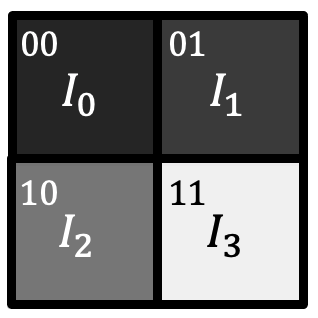
\includegraphics[width=0.5\columnwidth]{classical_repr.png}
		\caption{Rappresentazione di un'immagine B\&W 4x4 pixel.}
    \label{fig:bw-4x4-img}
\end{figure}

Per rappresentare l'immagine come una superposizione di stati base, è necessario
che venga rispettata l'Eq. \ref{eq:qubit-prob}; bisogna infatti normalizzare le singole intensità come segue:
\begin{equation}
	c_i = \frac{I_i}{\sqrt{\sum_{k}^{}{I_{k}^2}}}
	\label{eq:intensities-norm}
\end{equation}
In Fig. \ref{fig:bw-4x4-img-qpie}
viene mostrato il risultato della normalizzazione.
\begin{figure}[h!]
    \centering
    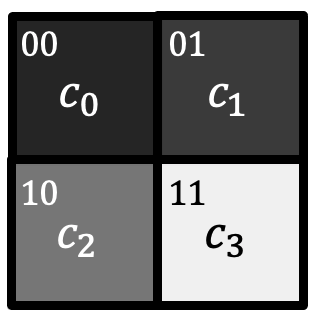
\includegraphics[width=0.5\columnwidth]{QPIE_repr.png}
		\caption{Rappresentazione della Fig. \ref{fig:bw-4x4-img} tramite QPIE.}
    \label{fig:bw-4x4-img-qpie}
\end{figure}

L'immagine può quindi essere scritta come:
\begin{equation*}
	\ket{\text{Img}}
		= c_0 \ket{00} + c_1 \ket{01} + c_2 \ket{10} + c_3 \ket{11}
	\label{eq:qpie-img-2qubit}
\end{equation*}
che generalizzata a $n$ qubit diventa:
\begin{equation}
	\ket{\text{Img}}
		= \sum_{i=1}^{2^n} c_i \ket{i}
	\label{eq:qpie-img}
\end{equation}


\subsection{Quantum Hadamard Edge Detection}

L'algoritmo di \textbf{Quantum Hadamard Edge Detection (QHED)} \cite{qpie} rappresenta il
fulcro di questo progetto. L'idea alla base è quella di utilizzare il gate di
Hadamard. Come mostrato nella Sottosez.
\ref{sec:img-rappr}, esso trasforma
$\ket{0}$ in $\ket{+}$ e, in particolare, $\ket{1}$ in $\ket{-}$. Inoltre, in
base alla Eq. \ref{eq:qpie-img}, ogni pixel può essere identificato
da una stringa binaria del tipo 
\[
	\ket{b_{n-1}b_{n-2}\ldots b_1b_0},\quad b_i \in {0,1}
\]
Per pixel orizzontalmente adiacenti presi a due a due, le stringhe sono:
\[
	\ket{b_{n-1}b_{n-2}\ldots b_10}, \ket{b_{n-1}b_{n-2}\ldots b_11}
\]
ossia si differenziano soltanto per l'ultimo qubit più a destra, denotato con $q_0$.

Applicando il gate $H$ a $q_0$, si ottiene una trasformazione la cui unitaria è
rappresentata da:
\begin{equation*}
	I_{2^{n-1}} \otimes H_0 = \frac{1}{\sqrt 2}\begin{bmatrix}
		1 & 1 & 0 & 0 & \ldots & 0 & 0\\
		1 & -1 & 0 & 0 & \ldots & 0 & 0\\
		0 & 0 & 1 & 1 & \ldots & 0 & 0\\
		0 & 0 & 1 & -1 & \ldots & 0 & 0\\
		\vdots & \vdots & \vdots & \vdots & \ddots & \vdots & \vdots\\
		0 & 0 & 0 & 0 & \ldots & 1 & 1\\
		0 & 0 & 0 & 0 & \ldots & 1 & -1\\
	\end{bmatrix}
\end{equation*}
Se a questo punto tale trasformazione è applicata allo stato che codifica
l'immagine nella notazione QPIE (Eq. \ref{eq:qpie-img}), si
ottiene:
\begin{equation}\label{eq:had-applied-simple}
	(I_{2^{n-1}} \otimes H_0) \cdot \begin{bmatrix}
		c_0\\ c_1\\ c_2\\ c_3\\ \vdots\\ c_{N-2}\\ c_{N-1}
	\end{bmatrix} = \frac{1}{\sqrt 2} \begin{bmatrix}
		c_0+c_1\\ c_0-c_1\\ c_2+c_3\\ c_2-c_3\\ \vdots\\ c_{N-2}+c_{N-1}\\ c_{N-2}-c_{N-1}
	\end{bmatrix}
\end{equation}
Si noti che ciò permette di esplicitare il gradiente di coppie di pixel adiacenti, in corrispondenza dei coefficienti in posizione \emph{dispari} nel vettore di stato risultante. Lo stato del'Eq. \ref{eq:had-applied-simple} può essere riscritto come:
\begin{align*}
	&\frac{1}{\sqrt 2} \begin{bmatrix}
	c_0+c_1\\ c_0-c_1\\ c_2+c_3\\ c_2-c_3\\ \vdots\\ c_{N-2}+c_{N-1}\\ c_{N-2}-c_{N-1}
\end{bmatrix}\\
	&=\frac{1}{\sqrt 2} 
\left(
\begin{bmatrix}
c_0+c_1\\ 0\\ c_2+c_3\\ 0\\ \vdots\\ c_{N-2}+c_{N-1}\\ 0
\end{bmatrix} + \begin{bmatrix}
0\\ c_0-c_1\\ 0\\ c_2-c_3\\ \vdots\\ 0\\ c_{N-2}-c_{N-1}
\end{bmatrix}
\right)\\
	&=\frac{1}{\sqrt 2} (\ket{\text{sum}} \otimes \ket{0}
		+ \ket{\text{dif}} \otimes \ket{1})
\end{align*}
da cui si evince che misurando il circuito condizionato sul fatto che $q_0$ sia nello stato $\ket{1}$, è possibile ottenere i gradienti attraverso un'analisi statistica.



\subsection{Modellazione del rumore}
